% Options for packages loaded elsewhere
\PassOptionsToPackage{unicode}{hyperref}
\PassOptionsToPackage{hyphens}{url}
\PassOptionsToPackage{dvipsnames,svgnames,x11names}{xcolor}
%
\documentclass[
  letterpaper,
  DIV=11,
  numbers=noendperiod]{scrartcl}

\usepackage{amsmath,amssymb}
\usepackage{lmodern}
\usepackage{iftex}
\ifPDFTeX
  \usepackage[T1]{fontenc}
  \usepackage[utf8]{inputenc}
  \usepackage{textcomp} % provide euro and other symbols
\else % if luatex or xetex
  \usepackage{unicode-math}
  \defaultfontfeatures{Scale=MatchLowercase}
  \defaultfontfeatures[\rmfamily]{Ligatures=TeX,Scale=1}
\fi
% Use upquote if available, for straight quotes in verbatim environments
\IfFileExists{upquote.sty}{\usepackage{upquote}}{}
\IfFileExists{microtype.sty}{% use microtype if available
  \usepackage[]{microtype}
  \UseMicrotypeSet[protrusion]{basicmath} % disable protrusion for tt fonts
}{}
\makeatletter
\@ifundefined{KOMAClassName}{% if non-KOMA class
  \IfFileExists{parskip.sty}{%
    \usepackage{parskip}
  }{% else
    \setlength{\parindent}{0pt}
    \setlength{\parskip}{6pt plus 2pt minus 1pt}}
}{% if KOMA class
  \KOMAoptions{parskip=half}}
\makeatother
\usepackage{xcolor}
\setlength{\emergencystretch}{3em} % prevent overfull lines
\setcounter{secnumdepth}{-\maxdimen} % remove section numbering
% Make \paragraph and \subparagraph free-standing
\ifx\paragraph\undefined\else
  \let\oldparagraph\paragraph
  \renewcommand{\paragraph}[1]{\oldparagraph{#1}\mbox{}}
\fi
\ifx\subparagraph\undefined\else
  \let\oldsubparagraph\subparagraph
  \renewcommand{\subparagraph}[1]{\oldsubparagraph{#1}\mbox{}}
\fi

\usepackage{color}
\usepackage{fancyvrb}
\newcommand{\VerbBar}{|}
\newcommand{\VERB}{\Verb[commandchars=\\\{\}]}
\DefineVerbatimEnvironment{Highlighting}{Verbatim}{commandchars=\\\{\}}
% Add ',fontsize=\small' for more characters per line
\usepackage{framed}
\definecolor{shadecolor}{RGB}{241,243,245}
\newenvironment{Shaded}{\begin{snugshade}}{\end{snugshade}}
\newcommand{\AlertTok}[1]{\textcolor[rgb]{0.68,0.00,0.00}{#1}}
\newcommand{\AnnotationTok}[1]{\textcolor[rgb]{0.37,0.37,0.37}{#1}}
\newcommand{\AttributeTok}[1]{\textcolor[rgb]{0.40,0.45,0.13}{#1}}
\newcommand{\BaseNTok}[1]{\textcolor[rgb]{0.68,0.00,0.00}{#1}}
\newcommand{\BuiltInTok}[1]{\textcolor[rgb]{0.00,0.23,0.31}{#1}}
\newcommand{\CharTok}[1]{\textcolor[rgb]{0.13,0.47,0.30}{#1}}
\newcommand{\CommentTok}[1]{\textcolor[rgb]{0.37,0.37,0.37}{#1}}
\newcommand{\CommentVarTok}[1]{\textcolor[rgb]{0.37,0.37,0.37}{\textit{#1}}}
\newcommand{\ConstantTok}[1]{\textcolor[rgb]{0.56,0.35,0.01}{#1}}
\newcommand{\ControlFlowTok}[1]{\textcolor[rgb]{0.00,0.23,0.31}{#1}}
\newcommand{\DataTypeTok}[1]{\textcolor[rgb]{0.68,0.00,0.00}{#1}}
\newcommand{\DecValTok}[1]{\textcolor[rgb]{0.68,0.00,0.00}{#1}}
\newcommand{\DocumentationTok}[1]{\textcolor[rgb]{0.37,0.37,0.37}{\textit{#1}}}
\newcommand{\ErrorTok}[1]{\textcolor[rgb]{0.68,0.00,0.00}{#1}}
\newcommand{\ExtensionTok}[1]{\textcolor[rgb]{0.00,0.23,0.31}{#1}}
\newcommand{\FloatTok}[1]{\textcolor[rgb]{0.68,0.00,0.00}{#1}}
\newcommand{\FunctionTok}[1]{\textcolor[rgb]{0.28,0.35,0.67}{#1}}
\newcommand{\ImportTok}[1]{\textcolor[rgb]{0.00,0.46,0.62}{#1}}
\newcommand{\InformationTok}[1]{\textcolor[rgb]{0.37,0.37,0.37}{#1}}
\newcommand{\KeywordTok}[1]{\textcolor[rgb]{0.00,0.23,0.31}{#1}}
\newcommand{\NormalTok}[1]{\textcolor[rgb]{0.00,0.23,0.31}{#1}}
\newcommand{\OperatorTok}[1]{\textcolor[rgb]{0.37,0.37,0.37}{#1}}
\newcommand{\OtherTok}[1]{\textcolor[rgb]{0.00,0.23,0.31}{#1}}
\newcommand{\PreprocessorTok}[1]{\textcolor[rgb]{0.68,0.00,0.00}{#1}}
\newcommand{\RegionMarkerTok}[1]{\textcolor[rgb]{0.00,0.23,0.31}{#1}}
\newcommand{\SpecialCharTok}[1]{\textcolor[rgb]{0.37,0.37,0.37}{#1}}
\newcommand{\SpecialStringTok}[1]{\textcolor[rgb]{0.13,0.47,0.30}{#1}}
\newcommand{\StringTok}[1]{\textcolor[rgb]{0.13,0.47,0.30}{#1}}
\newcommand{\VariableTok}[1]{\textcolor[rgb]{0.07,0.07,0.07}{#1}}
\newcommand{\VerbatimStringTok}[1]{\textcolor[rgb]{0.13,0.47,0.30}{#1}}
\newcommand{\WarningTok}[1]{\textcolor[rgb]{0.37,0.37,0.37}{\textit{#1}}}

\providecommand{\tightlist}{%
  \setlength{\itemsep}{0pt}\setlength{\parskip}{0pt}}\usepackage{longtable,booktabs,array}
\usepackage{calc} % for calculating minipage widths
% Correct order of tables after \paragraph or \subparagraph
\usepackage{etoolbox}
\makeatletter
\patchcmd\longtable{\par}{\if@noskipsec\mbox{}\fi\par}{}{}
\makeatother
% Allow footnotes in longtable head/foot
\IfFileExists{footnotehyper.sty}{\usepackage{footnotehyper}}{\usepackage{footnote}}
\makesavenoteenv{longtable}
\usepackage{graphicx}
\makeatletter
\def\maxwidth{\ifdim\Gin@nat@width>\linewidth\linewidth\else\Gin@nat@width\fi}
\def\maxheight{\ifdim\Gin@nat@height>\textheight\textheight\else\Gin@nat@height\fi}
\makeatother
% Scale images if necessary, so that they will not overflow the page
% margins by default, and it is still possible to overwrite the defaults
% using explicit options in \includegraphics[width, height, ...]{}
\setkeys{Gin}{width=\maxwidth,height=\maxheight,keepaspectratio}
% Set default figure placement to htbp
\makeatletter
\def\fps@figure{htbp}
\makeatother
\newlength{\cslhangindent}
\setlength{\cslhangindent}{1.5em}
\newlength{\csllabelwidth}
\setlength{\csllabelwidth}{3em}
\newlength{\cslentryspacingunit} % times entry-spacing
\setlength{\cslentryspacingunit}{\parskip}
\newenvironment{CSLReferences}[2] % #1 hanging-ident, #2 entry spacing
 {% don't indent paragraphs
  \setlength{\parindent}{0pt}
  % turn on hanging indent if param 1 is 1
  \ifodd #1
  \let\oldpar\par
  \def\par{\hangindent=\cslhangindent\oldpar}
  \fi
  % set entry spacing
  \setlength{\parskip}{#2\cslentryspacingunit}
 }%
 {}
\usepackage{calc}
\newcommand{\CSLBlock}[1]{#1\hfill\break}
\newcommand{\CSLLeftMargin}[1]{\parbox[t]{\csllabelwidth}{#1}}
\newcommand{\CSLRightInline}[1]{\parbox[t]{\linewidth - \csllabelwidth}{#1}\break}
\newcommand{\CSLIndent}[1]{\hspace{\cslhangindent}#1}

\KOMAoption{captions}{tableheading}
\makeatletter
\makeatother
\makeatletter
\makeatother
\makeatletter
\@ifpackageloaded{caption}{}{\usepackage{caption}}
\AtBeginDocument{%
\ifdefined\contentsname
  \renewcommand*\contentsname{Table of contents}
\else
  \newcommand\contentsname{Table of contents}
\fi
\ifdefined\listfigurename
  \renewcommand*\listfigurename{List of Figures}
\else
  \newcommand\listfigurename{List of Figures}
\fi
\ifdefined\listtablename
  \renewcommand*\listtablename{List of Tables}
\else
  \newcommand\listtablename{List of Tables}
\fi
\ifdefined\figurename
  \renewcommand*\figurename{Figure}
\else
  \newcommand\figurename{Figure}
\fi
\ifdefined\tablename
  \renewcommand*\tablename{Table}
\else
  \newcommand\tablename{Table}
\fi
}
\@ifpackageloaded{float}{}{\usepackage{float}}
\floatstyle{ruled}
\@ifundefined{c@chapter}{\newfloat{codelisting}{h}{lop}}{\newfloat{codelisting}{h}{lop}[chapter]}
\floatname{codelisting}{Listing}
\newcommand*\listoflistings{\listof{codelisting}{List of Listings}}
\makeatother
\makeatletter
\@ifpackageloaded{caption}{}{\usepackage{caption}}
\@ifpackageloaded{subcaption}{}{\usepackage{subcaption}}
\makeatother
\makeatletter
\@ifpackageloaded{tcolorbox}{}{\usepackage[many]{tcolorbox}}
\makeatother
\makeatletter
\@ifundefined{shadecolor}{\definecolor{shadecolor}{rgb}{.97, .97, .97}}
\makeatother
\makeatletter
\makeatother
\ifLuaTeX
  \usepackage{selnolig}  % disable illegal ligatures
\fi
\IfFileExists{bookmark.sty}{\usepackage{bookmark}}{\usepackage{hyperref}}
\IfFileExists{xurl.sty}{\usepackage{xurl}}{} % add URL line breaks if available
\urlstyle{same} % disable monospaced font for URLs
\hypersetup{
  pdftitle={Bootstrapping},
  pdfauthor={Caelan Bryan; Jenna Dufresne; Jamielee Jimenez Perez},
  colorlinks=true,
  linkcolor={blue},
  filecolor={Maroon},
  citecolor={Blue},
  urlcolor={Blue},
  pdfcreator={LaTeX via pandoc}}

\title{Bootstrapping}
\author{Caelan Bryan \and Jenna Dufresne \and Jamielee Jimenez Perez}
\date{11/22/22}

\begin{document}
\maketitle
\ifdefined\Shaded\renewenvironment{Shaded}{\begin{tcolorbox}[interior hidden, enhanced, frame hidden, borderline west={3pt}{0pt}{shadecolor}, breakable, boxrule=0pt, sharp corners]}{\end{tcolorbox}}\fi

View presentation \href{/Bootstrapping-Group-Presentation.html}{here}

\hypertarget{introduction}{%
\subsection{Introduction}\label{introduction}}

Resampling is the process of creating new samples based on an observed
sample to gather more information about either the sample or the
population the sample came from. Resampling techniques like permutation
tests, cross validation, and the jackknife have been prevalent in the
statistics world for a while.

Resampling can come in handy when it's either impossible or unfeasible
to retrieve a sample from the entire population. For instance, if you
wanted to learn more about all attendees of a concert it would be very
difficult to survey every single person in attendance. While you might
not be able to survey everyone at the concert, you most likely could
survey a smaller subset, say 100 to 200. With resampling techniques you
could verify the accuracy of the original sample, or make observations
about the entire population of concert goers.

All of the resampling techniques listed either have assumptions required
for them to make meaningful results, fail at specific estimations, or
produce errors during the process. The Bootstrap method was introduced
to overcome some of the pitfalls of the jackknife resampling method.

\hypertarget{what-is-the-bootstrap-method}{%
\subsubsection{What is the Bootstrap
Method}\label{what-is-the-bootstrap-method}}

The Bootstrap Method was first introduced by Bradley Efron in Bootstrap
Methods: Another Look at the Jackknife (B. Efron 1979). He described the
Bootstrap as a more primitive method, whose applications are more wide
and dependable than those of the jackknife. The Bootstrap was introduced
as a way to estimate a sampling distribution based on the observed
sample. The Bootstrap is also shown to estimate the variance here, which
is an area the jackknife fails at, along with being shown to do well as
estimated the error rates in certain problems, outperforming other
non-parametric estimation methods.

At a very high-level, Bootstrapping is the process of taking a sample
and using it to create a new sample with replacement. Doing so gives
every observation an equal chance to show up in the new sample, and some
might show up more than once while others might not show up due to
replacement. Doing this multiple times can give an understanding about
the population that the original sample came from.

While all Bootstrap methods follow the same formula, there are some
slight differences between different version of the Bootstrap. For
example, the Monte Carlo technique takes exact copies of the data from
the original sample to place into the new sample (Hossain 2000) while
the Bayesian Bootstrap adds weights to each observation before selecting
the data for the new sample. These slight differences result in multiple
different types of Bootstraps that can be used for different
applications or to get around certain assumptions of another type of
Bootstrap.

\hypertarget{assumptions-and-shortcomings}{%
\subsubsection{Assumptions and
Shortcomings}\label{assumptions-and-shortcomings}}

As Bootstrapping gains popularity, it's important to understand that
there are still assumptions that must be met, and shortcomings that
should be understood. The Importance of Discussing Assumptions when
Teaching Bootstrapping (Totty, Molyneux, and Fuentes 2021) takes an
interesting approach of looking at those who are learning about
Bootstrapping, and assessing possible pain points. The largest
assumption listed is that the distribution can be made approximately
pivotal through shifting or studentization. Further in this paper, an
interesting result came out that if assumptions are broken when
performing the Bootstrap method, it performs no better or worse then
other methods whose assumptions are also broken. Performing
Bootstrapping with broken assumptions can also lead to decreased
performance of the method.

One of the shortcomings of the Bootstrap method is that the results
still rely on the original sample (Hossain 2000). So, if the original
sample contains many outliers, then it most likely won't produce an
accurate representation of the population. Small sample sizes and data
that does not follow a normal distribution has also been found to
negatively impact the performance of Bootstrapping methods (Totty,
Molyneux, and Fuentes 2021).

\hypertarget{applications}{%
\subsubsection{Applications}\label{applications}}

Bootstrapping has far reaching applications from finding a population
mean to performing hypothesis testing. Initially, Efron introduced the
Bootstrap method to estimate the sampling distribution, estimate the
median, error rate estimation in discrimination analysis, Wilcoxon's
statistic, and regression models (B. Efron 1979). Another application
from Efron was introduced in Nonparametric Estimates of Standard Error:
The Jackknife, the Bootstrap, and Other Methods (Bradley Efron 1981). He
introduces the concept of using the Bootstrap to estimate the standard
error based on the data. While this is normally done using parametric
modeling methods, here it is being done with non-parametric methods,
like the Bootstrap. As time has progressed, and computers have become
more powerful, the applications of Bootstrapping have increased.

One popular application is using Bootstrapping to create confidence
intervals for certain statistics. Due to the nature of Bootstrapping, it
creates results that make perfect sense to construct confidence
intervals. Often, Bootstrapping implements confidence intervals around
estimated parameter values (Puth, Neuhäuser, and Ruxton 2015). One
example is using Bootstrapping to find the population mean of a specific
feature based on the sample means. A few other similar applications are
creating a confidence interval for the population mean and estimating
the distribution of a sample mean (Hossain 2000).

Another popular application to Bootstrapping is in regression. In
regression, the Bootstrap method can be used to perform validation on
the model. In Bootstrapping with R to make generalized inference for
regression model (Sillabutra et al. 2016) the authors used the Bootstrap
method to resample thousands of times, fit a model to each new sample,
and save the intercept and regression coefficient estimates. Confidence
intervals can then be created to assess performance of a population
regression model against the Bootstrap sample models. Another possible
application of Bootstrapping in regression is using it to approximate
the distribution of the Lasso estimator for all possible values of the
unknown regression parameter vector (Chatterjee and Lahiri 2011). The
residual bootstrap can also be used to consistently estimate the
distribution and variance of the adaptive Lasso estimator.

The rise of statistical and mathematical programming languages and tools
have greatly improved the state of Bootstrapping. Since Bootstrapping
normally requires a large number of iterations to produce meaningful
results, faster computers and tools have allowed statisticians to gain
useful information. software packages have been created for SAS, Stata
(MD et al. 2005), and R (Sillabutra et al. 2016) that allow common
Bootstrapping functionality to be used readily and easily.

\hypertarget{methods}{%
\subsection{Methods}\label{methods}}

There are a variety of different Bootstrap methods for specific
scenarios, populations, samples, and applications. Although, many of the
Bootstrap methods follow a similar set of steps. These steps for the
one-sample problem were outlined in Bootstrap Methods: Another Look at
the Jackknife (B. Efron 1979)

\begin{enumerate}
\def\labelenumi{\arabic{enumi}.}
\tightlist
\item
  Construct the sample probability distribution \(\hat{F}\), putting
  mass \(1/n\) at each point \(x_1, x_2, x_3, . . . , x_n\).
\item
  With \(\hat{F}\) fixed, draw a random sample of size \(n\) from
  \(\hat{F}\), say \(X_{i}^{*} = x_{i}^{*}\),
  \(X_{i}^{*} \sim _{ind}\hat{F}\) and call this the bootstrap sample.
\item
  Approximate the sampling distribution of \(R(X, \hat{F}\) by the
  bootstrap distribution of \(R^{*} = R(X^{*}, \hat{F})\).
\end{enumerate}

Or more simply, to perform the Bootstrap method as proposed, given a
sample of size \(n\), a new sample of size \(n\) can be created by
selecting from the original sample with replacement. Since the new
sample is created with replacement, every element from the original
sample has the same probability of ending up in the new sample. This can
then by performed multiple times to estimate the sampling distribution
based on the Bootstrap distribution.

As time went on, new methods for Bootstrapping were introduced to be
applied to different applications or to further enhance the accuracy.
Some of the more popular methods are listed below.

\hypertarget{types-of-bootstrap}{%
\subsubsection{Types of Bootstrap}\label{types-of-bootstrap}}

\textbf{Monte Carlo Case resampling}

In the Monte Carlo method, a new sample is created by randomly selecting
values from the original sample using replacement to create a sample of
the same size. Statistics can then be computed from this new sample.
This process is then repeated many times to create an estimate of the
population statistic. (B. Efron 1979)

\textbf{Exact Case resampling}

The exact version for Bootstrap case resampling is similar to the Monte
Carlo method, except every possible enumeration of the initial sample is
created. The downside to this method is since there are a total of
\({2n - 1 \choose n} = \frac{(2n - 1)!}{n!(n - 1)!}\) possible samples,
the process can be very intensive for large sample sizes. (Hossain 2000)

\textbf{Smooth Bootstrap}

In the Smooth Bootstrap, a small amount of random noise is added to
every re-sampled observation. This noise is zero-centered and usually
normally distributed. Doing this means that the re-sampled data is not
limited to just the data in the original sample, but rather to data
points in close proximity to the original samples. Figure~\ref{fig-1}
shows an example of the simple bootstrap density function and
Figure~\ref{fig-2} shows an example of the smoothed density function
provided by (Dwornicka, Goroshko, and Pietraszek 2019).

\begin{figure}

\begin{minipage}[t]{0.50\linewidth}

{\centering 

\raisebox{-\height}{

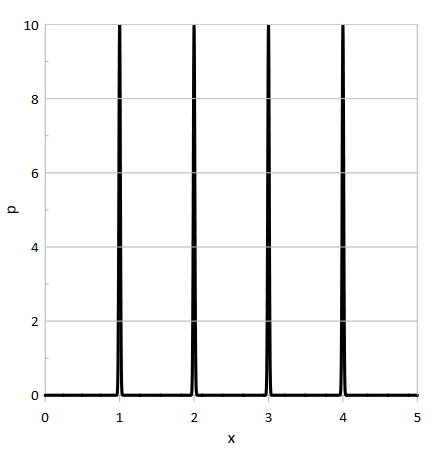
\includegraphics{Bootstrapping-Group-Report_files/figure-html/smooth1.png}

}

\caption{\label{fig-1}Simple Bootstrap Density Function}

}

\end{minipage}%
%
\begin{minipage}[t]{0.50\linewidth}

{\centering 

\raisebox{-\height}{

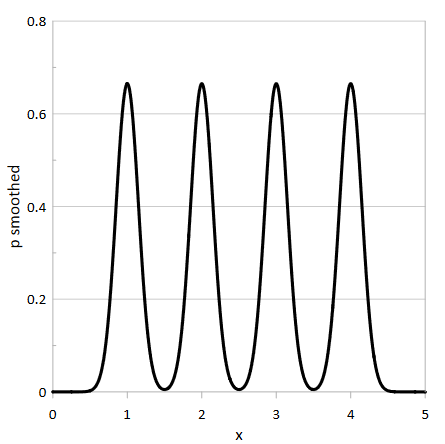
\includegraphics{Bootstrapping-Group-Report_files/figure-html/smooth2.png}

}

\caption{\label{fig-2}Smoothed Bootstrap Density Function}

}

\end{minipage}%

\end{figure}

While these are some of the more popular methods for Bootstrapping,
since Bootstrapping simply refers to a test that uses random sampling
with replacement, there are multiple other types of Bootstrap methods.
Some others include the Bayesian Bootstrap method, which creates new
samples through assigning weights to the original data (Rubin 1981), the
Parametric Bootstrap, the Poisson Bootstrap, the Block Bootstrap, and
resampling residuals.

\hypertarget{analysis-and-results}{%
\subsection{Analysis and Results}\label{analysis-and-results}}

\hypertarget{data-and-visualization}{%
\subsubsection{Data and Visualization}\label{data-and-visualization}}

\hypertarget{initial-data-sets}{%
\paragraph{Initial Data Sets}\label{initial-data-sets}}

The dataset being used to explore Bootstrapping is the ``Causes of Death
- Our World in Data'' dataset from Kaggle (Chavez 2022) which was
expanded with the World Bank population dataset (2022). The ``Causes of
Death - Our World in Data'' dataset contains thirty three causes of
death broken down by continent, region, country, and territory and by
the year of reporting. The World Bank population dataset contains
population numbers for multiple years also broken down by continent,
region, country, and territory. The populations from the population
dataset were added into the causes of death dataset to allow for the
calculation of the rate of death, or percentage of total population, for
each cause of death.

To complete the original dataset, all rows that did not correspond to
countries were removed. The number of executions and terrorism columns
were also removed from the original causes of death dataset due to a
lack of data for most countries.

As a final note, the Vatican and Liechtenstein are the only two
countries missing from the final, cleaned, dataset because they were not
included in the original causes of death dataset from Kaggle.

\begin{Shaded}
\begin{Highlighting}[]
\CommentTok{\# Import the data}
\NormalTok{bootstrapping\_data\_cleaned }\OtherTok{=} \FunctionTok{read.csv}\NormalTok{(}\StringTok{\textquotesingle{}bootstrapping\_data\_cleaned.csv\textquotesingle{}}\NormalTok{, }
                                      \AttributeTok{stringsAsFactors =} \ConstantTok{TRUE}\NormalTok{)}
\end{Highlighting}
\end{Shaded}

\hypertarget{data-cleaning}{%
\paragraph{Data Cleaning}\label{data-cleaning}}

In order to fit the data into the experiments introduced later in the
paper, the dataset will need to be further modified. A new column,
Number\_Of\_Deaths, that includes the total number of reported deaths
for a specific country and year by adding together the totals from all
causes of deaths will be added. Next, only the columns needed for the
experiments are extracted into a new dataset called boot\_data. At this
point, only data from the most recent reported year, 2019, is also
extracted. The columns needed are the Entity, Population,
Number\_of\_Deaths, Deaths\_cardiovascularDiseases, and
Deaths\_InterpersonalViolence columns. Lastly, a new column is created
that is the rate of all deaths caused by cardiovascular diseases.

\begin{Shaded}
\begin{Highlighting}[]
\CommentTok{\# Create the total number of reported deaths column}
\NormalTok{bootstrapping\_data\_cleaned}\SpecialCharTok{$}\NormalTok{Number\_Of\_Deaths }\OtherTok{\textless{}{-}} 
  \FunctionTok{rowSums}\NormalTok{(bootstrapping\_data\_cleaned[,(}\DecValTok{5}\SpecialCharTok{:}\DecValTok{35}\NormalTok{)])}

\CommentTok{\# Filter down the data to just include 2019 and just the columns needed}
\NormalTok{boot\_data }\OtherTok{=} 
\NormalTok{  bootstrapping\_data\_cleaned[bootstrapping\_data\_cleaned}\SpecialCharTok{$}\NormalTok{Year }\SpecialCharTok{==} \StringTok{\textquotesingle{}2019\textquotesingle{}}\NormalTok{, }
                             \FunctionTok{c}\NormalTok{(}\StringTok{\textquotesingle{}Entity\textquotesingle{}}\NormalTok{, }\StringTok{\textquotesingle{}Population\textquotesingle{}}\NormalTok{, }\StringTok{\textquotesingle{}Number\_Of\_Deaths\textquotesingle{}}\NormalTok{,}
                               \StringTok{\textquotesingle{}Deaths\_CardiovascularDiseases\textquotesingle{}}\NormalTok{,}
                               \StringTok{\textquotesingle{}Deaths\_InterpersonalViolence\textquotesingle{}}\NormalTok{)]}

\CommentTok{\# Create the cardiovascular diseases rate column}
\NormalTok{boot\_data}\SpecialCharTok{$}\NormalTok{Deaths\_CardiovascularDiseasesRate }\OtherTok{\textless{}{-}} 
\NormalTok{  boot\_data}\SpecialCharTok{$}\NormalTok{Deaths\_CardiovascularDiseases }\SpecialCharTok{/}\NormalTok{ boot\_data}\SpecialCharTok{$}\NormalTok{Number\_Of\_Deaths}
\end{Highlighting}
\end{Shaded}

The dataset now contains the following columns:

\begin{longtable}[]{@{}
  >{\raggedright\arraybackslash}p{(\columnwidth - 4\tabcolsep) * \real{0.3889}}
  >{\raggedright\arraybackslash}p{(\columnwidth - 4\tabcolsep) * \real{0.3611}}
  >{\raggedright\arraybackslash}p{(\columnwidth - 4\tabcolsep) * \real{0.2500}}@{}}
\toprule()
\begin{minipage}[b]{\linewidth}\raggedright
Name
\end{minipage} & \begin{minipage}[b]{\linewidth}\raggedright
Description
\end{minipage} & \begin{minipage}[b]{\linewidth}\raggedright
Type
\end{minipage} \\
\midrule()
\endhead
Entity & Name of Country & Nominal \\
Population & Population of Country in 2019 & Discrete \\
Number\_of\_Deaths & Total Number of Deaths for Country in 2019 &
Discrete \\
Deaths\_CardiovascularDiseases & Total Number of Deaths for Country
Caused by Cardiovascular Diseases in 2019 & Nominal \\
Deaths\_InterpersonalViolence & Total Number of Deaths for Country
Caused by Interpersonal Violence in 2019 & Discrete \\
Deaths\_CardiovascularDiseasesRate & Rate of Deaths in Country Caused by
Cardiovascular Diseases in 2019 & Continuous \\
\bottomrule()
\end{longtable}

\hypertarget{descriptive-statistics}{%
\paragraph{Descriptive Statistics}\label{descriptive-statistics}}

Now that the dataset is created, we can find population descriptive
statistics to compare against the estimated population statistics from
Bootstrapping. The data can also be visualized to check that the rate of
deaths caused by cardiovascular diseases follows a normal distribution
and that there appears to be a relationship between the number of deaths
caused by interpersonal violence and the population of a country.

\begin{Shaded}
\begin{Highlighting}[]
\CommentTok{\# Find cardiovascular disease death rate statistics}
\NormalTok{boot\_means }\OtherTok{\textless{}{-}}\NormalTok{ boot\_data }\SpecialCharTok{\%\textgreater{}\%} \FunctionTok{summarize}\NormalTok{(}\AttributeTok{mean\_cardiovasculardiseasesrate =} 
                                        \FunctionTok{mean}\NormalTok{(Deaths\_CardiovascularDiseasesRate),}
                                      \AttributeTok{sd\_cardiovasculardiseasesrate =} 
                                        \FunctionTok{sd}\NormalTok{(Deaths\_CardiovascularDiseasesRate))}
\end{Highlighting}
\end{Shaded}

The average rate of deaths caused by cardiovascular diseases across the
entire population is 0.3273, or 32.73\%, with a standard deviation of
0.1309, or 13.09\%.

\begin{Shaded}
\begin{Highlighting}[]
\CommentTok{\# Create a histogram of the cardiovascular diseases death rate}
\NormalTok{cardioHistogram }\OtherTok{\textless{}{-}} \FunctionTok{ggplot}\NormalTok{(boot\_data, }
                          \FunctionTok{aes}\NormalTok{(}\AttributeTok{x =}\NormalTok{ Deaths\_CardiovascularDiseasesRate)) }\SpecialCharTok{+}
                   \FunctionTok{xlab}\NormalTok{(}\StringTok{\textquotesingle{}Cardiovascular Diseases Death Rate\textquotesingle{}}\NormalTok{) }\SpecialCharTok{+}
                   \FunctionTok{ylab}\NormalTok{(}\StringTok{\textquotesingle{}Count\textquotesingle{}}\NormalTok{) }\SpecialCharTok{+}
                   \FunctionTok{geom\_histogram}\NormalTok{()}

\CommentTok{\# Create a histogram of the interpersonal violence death rate}
\NormalTok{violenceHistogram }\OtherTok{\textless{}{-}} \FunctionTok{ggplot}\NormalTok{(boot\_data, }
                            \FunctionTok{aes}\NormalTok{(}\AttributeTok{x =}\NormalTok{ Deaths\_InterpersonalViolence, }
                                \AttributeTok{y =}\NormalTok{ Population)) }\SpecialCharTok{+}
                     \FunctionTok{scale\_x\_log10}\NormalTok{() }\SpecialCharTok{+}
                     \FunctionTok{scale\_y\_log10}\NormalTok{() }\SpecialCharTok{+}
                     \FunctionTok{xlab}\NormalTok{(}\StringTok{\textquotesingle{}Interpersonal Violence Deaths (log 10)\textquotesingle{}}\NormalTok{) }\SpecialCharTok{+}
                     \FunctionTok{ylab}\NormalTok{(}\StringTok{\textquotesingle{}Population (log 10)\textquotesingle{}}\NormalTok{) }\SpecialCharTok{+}
                     \FunctionTok{geom\_point}\NormalTok{() }

\CommentTok{\# Display plots side by side}
\FunctionTok{grid.arrange}\NormalTok{(cardioHistogram, violenceHistogram, }\AttributeTok{ncol =} \DecValTok{2}\NormalTok{)}
\end{Highlighting}
\end{Shaded}

\begin{figure}[H]

{\centering 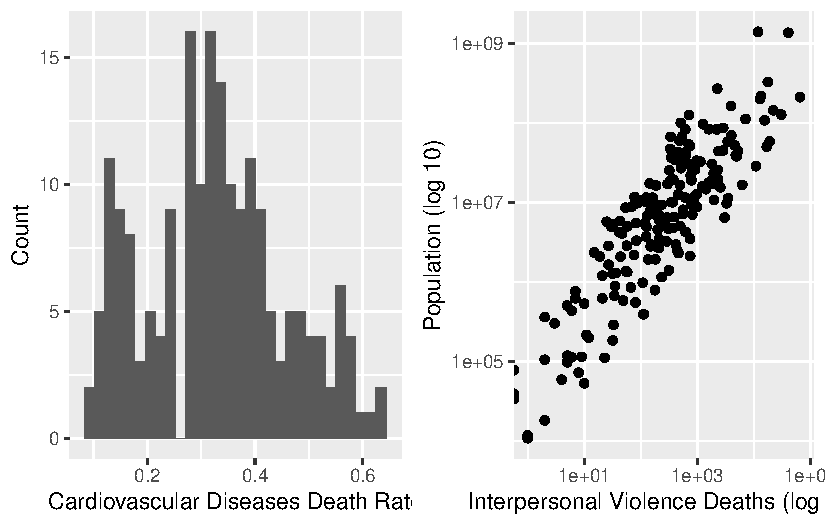
\includegraphics{Bootstrapping-Group-Report_files/figure-pdf/unnamed-chunk-8-1.pdf}

}

\end{figure}

Based on the histogram for the cardiovascular diseases death rate, it
appears that the death rate for cardiovascular diseases may follow a
normal distribution. The plot for interpersonal violence shows that
there may be a relationship between the number of deaths caused by
interpersonal violence and the population of the country. In both cases
the data appear to be good contenders for statistical modeling using the
Bootstrap method.

\hypertarget{statistical-modeling}{%
\subsubsection{Statistical Modeling}\label{statistical-modeling}}

Two applications of the Bootstrap method, both using the Monte Carlo
method (new samples are the exact size as the original sample) will be
analyzed. The first application is estimating the population mean and
standard deviation of the cardiovascular diseases death rate. The second
application is testing the variability of a simple linear regression
model that estimates the number of interpersonal violence deaths on the
population of a country.

In both experiments a sample of the full population data will need to be
taken to continue with the Bootstrap applications. A sample of the
population was taken, without replacement, with size \(n = 20\) to use
in the two applications.

\begin{Shaded}
\begin{Highlighting}[]
\CommentTok{\# Create the initial sample}
\NormalTok{boot\_initial\_sample }\OtherTok{\textless{}{-}} \FunctionTok{sample}\NormalTok{(}\DecValTok{1}\SpecialCharTok{:}\FunctionTok{nrow}\NormalTok{(boot\_data), }\DecValTok{20}\NormalTok{, }\AttributeTok{replace =} \ConstantTok{FALSE}\NormalTok{)}
\end{Highlighting}
\end{Shaded}

\hypertarget{estimating-population-mean-and-standard-deviation}{%
\paragraph{Estimating Population Mean and Standard
Deviation}\label{estimating-population-mean-and-standard-deviation}}

To estimate the population mean and standard deviation using the
Bootstrap method, 1,000 new samples were created, with replacement,
using the initial sample created. A simple loop can be created to
continuously create these new samples. For every new sample that is
created, the mean and standard deviation can be calculated and saved to
be analyzed.

\begin{Shaded}
\begin{Highlighting}[]
\CommentTok{\# Create vectors to store new sample means and standard deviations}
\NormalTok{boot\_estimated\_means }\OtherTok{\textless{}{-}} \FunctionTok{rep}\NormalTok{()}
\NormalTok{boot\_estimated\_sds }\OtherTok{\textless{}{-}} \FunctionTok{rep}\NormalTok{()}
\CommentTok{\# Create 1,000 new samples and save the means and standard deviations}
\ControlFlowTok{for}\NormalTok{ (x }\ControlFlowTok{in} \DecValTok{1}\SpecialCharTok{:}\DecValTok{1000}\NormalTok{) \{}
\NormalTok{  boot\_new\_sample }\OtherTok{\textless{}{-}} \FunctionTok{sample}\NormalTok{(boot\_initial\_sample, }\DecValTok{20}\NormalTok{, }\AttributeTok{replace =} \ConstantTok{TRUE}\NormalTok{)}
\NormalTok{  boot\_estimated\_means }\OtherTok{\textless{}{-}} \FunctionTok{append}\NormalTok{(boot\_estimated\_means,}
                                 \FunctionTok{pull}\NormalTok{(}
                                   \FunctionTok{summarize}\NormalTok{(}
\NormalTok{                                     boot\_data[boot\_new\_sample,], }
                                     \FunctionTok{mean}\NormalTok{(Deaths\_CardiovascularDiseasesRate))))}
\NormalTok{  boot\_estimated\_sds }\OtherTok{\textless{}{-}} \FunctionTok{append}\NormalTok{(boot\_estimated\_sds, }
                               \FunctionTok{pull}\NormalTok{(}
                                 \FunctionTok{summarize}\NormalTok{(}
\NormalTok{                                   boot\_data[boot\_new\_sample,], }
                                   \FunctionTok{sd}\NormalTok{(Deaths\_CardiovascularDiseasesRate))))}
\NormalTok{\}}
\end{Highlighting}
\end{Shaded}

\begin{Shaded}
\begin{Highlighting}[]
\CommentTok{\# Display some estimated means}
\FunctionTok{head}\NormalTok{(boot\_estimated\_means)}
\end{Highlighting}
\end{Shaded}

\begin{verbatim}
[1] 0.3018411 0.2960189 0.2528286 0.2768492 0.2906119 0.2408266
\end{verbatim}

\begin{Shaded}
\begin{Highlighting}[]
\CommentTok{\# Display some estimated standard deviations}
\FunctionTok{head}\NormalTok{(boot\_estimated\_sds)}
\end{Highlighting}
\end{Shaded}

\begin{verbatim}
[1] 0.08163061 0.09082884 0.09021657 0.09568397 0.07292899 0.08355213
\end{verbatim}

In order to create a 95\% confidence interval for the population mean
and standard deviation, the top and bottom 2.5\% of saved means and
standard deviations can be trimmed.

\begin{Shaded}
\begin{Highlighting}[]
\CommentTok{\# Sort the estimated means from smallest to largest}
\NormalTok{boot\_estimated\_means }\OtherTok{\textless{}{-}} \FunctionTok{sort}\NormalTok{(boot\_estimated\_means)}
\CommentTok{\# Sort the estimated standard deviations from smallest to largest}
\NormalTok{boot\_estimated\_sds }\OtherTok{\textless{}{-}} \FunctionTok{sort}\NormalTok{(boot\_estimated\_sds)}
\CommentTok{\# Trim the top and bottom 2.5\%}
\NormalTok{start }\OtherTok{=} \FunctionTok{length}\NormalTok{(boot\_estimated\_means) }\SpecialCharTok{*} \FloatTok{0.025}
\NormalTok{end }\OtherTok{=} \FunctionTok{length}\NormalTok{(boot\_estimated\_means) }\SpecialCharTok{*} \FloatTok{0.975}
\NormalTok{boot\_estimated\_means }\OtherTok{\textless{}{-}}\NormalTok{ boot\_estimated\_means[start}\SpecialCharTok{:}\NormalTok{end]}
\NormalTok{boot\_estimated\_sds }\OtherTok{\textless{}{-}}\NormalTok{ boot\_estimated\_sds[start}\SpecialCharTok{:}\NormalTok{end]}
\end{Highlighting}
\end{Shaded}

Now, by retrieving the first and last element in both the mean and
standard deviation vectors, the 95\% estimated population intervals can
be constructed. The 95\% confidence interval for the population mean is
{[}0.2428, 0.3205{]} or {[}24.28\%, 32.05\%{]}. The 95\% confidence
interval for the population standard deviation is {[}0.0698, 0.1041{]}
or {[}6.98\%, 10.41\%{]}.

To evaluate the accuracy of the estimated population mean and standard
deviation for the rate of deaths caused by cardiovascular diseases, the
population mean and standard deviation found from the full population
can be compared to the estimated confidence intervals. The true
population statistics should fall within the confidence interval range.
In this case:

\(0.2428 > 0.3273 > 0.3205\)

\(0.0698 > 0.1309 > 0.1041\)

\begin{Shaded}
\begin{Highlighting}[]
\CommentTok{\# Display a histogram of the estimated means from the Bootstrap samples}
\FunctionTok{ggplot}\NormalTok{() }\SpecialCharTok{+}
\FunctionTok{geom\_histogram}\NormalTok{(}\FunctionTok{aes}\NormalTok{(boot\_estimated\_means))}
\end{Highlighting}
\end{Shaded}

\begin{figure}[H]

{\centering 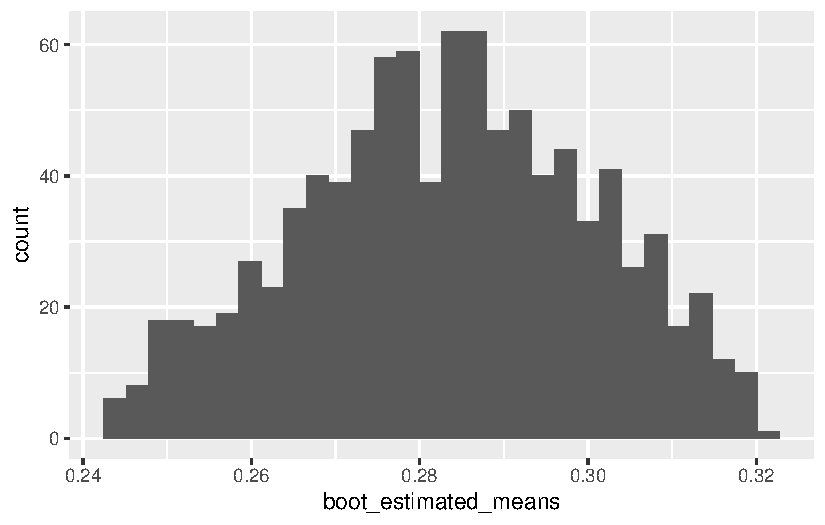
\includegraphics{Bootstrapping-Group-Report_files/figure-pdf/unnamed-chunk-18-1.pdf}

}

\end{figure}

Visualizing the estimated means shows that they follow a normal
distribution. This matches the full population data for the rate of
deaths caused by cardiovascular diseases, which also follows a normal
distribution.

\hypertarget{finding-variablility-of-regression-model}{%
\paragraph{Finding Variablility of Regression
Model}\label{finding-variablility-of-regression-model}}

The next experiment is finding the variability for a simple linear
regression model. For this experiment a model will be fit that estimates
the number of deaths caused by interpersonal violence by the population
of a country. Similar to the first experiment, 1,000 new samples will be
created and analyzed, except instead of retrieving the mean and standard
deviation, a linear regression model will be fit based on the new sample
and the intercept and regression parameter will be extracted and saved.

\begin{Shaded}
\begin{Highlighting}[]
\CommentTok{\# Create vectors to store new intercepts and regression parameters}
\NormalTok{boot\_estimated\_intercepts }\OtherTok{\textless{}{-}} \FunctionTok{rep}\NormalTok{()}
\NormalTok{boot\_estimated\_regressionparameters }\OtherTok{\textless{}{-}} \FunctionTok{rep}\NormalTok{()}
\CommentTok{\# Create 1,000 new samples and save the means and standard deviations}
\ControlFlowTok{for}\NormalTok{ (x }\ControlFlowTok{in} \DecValTok{1}\SpecialCharTok{:}\DecValTok{1000}\NormalTok{) \{}
\NormalTok{  boot\_new\_reg\_sample }\OtherTok{\textless{}{-}} \FunctionTok{sample}\NormalTok{(boot\_initial\_sample, }\DecValTok{20}\NormalTok{, }\AttributeTok{replace =} \ConstantTok{TRUE}\NormalTok{)}
\NormalTok{  boot\_new\_lm }\OtherTok{\textless{}{-}} \FunctionTok{lm}\NormalTok{(Deaths\_InterpersonalViolence }\SpecialCharTok{\textasciitilde{}}\NormalTok{ Population,}
\NormalTok{                    boot\_data[boot\_new\_reg\_sample,])}
\NormalTok{  boot\_estimated\_intercepts }\OtherTok{\textless{}{-}} \FunctionTok{append}\NormalTok{(boot\_estimated\_intercepts, }
\NormalTok{                                      boot\_new\_lm}\SpecialCharTok{$}\NormalTok{coefficients[}\DecValTok{1}\NormalTok{])}
\NormalTok{  boot\_estimated\_regressionparameters }\OtherTok{\textless{}{-}} 
    \FunctionTok{append}\NormalTok{(boot\_estimated\_regressionparameters, }
\NormalTok{           boot\_new\_lm}\SpecialCharTok{$}\NormalTok{coefficients[}\DecValTok{2}\NormalTok{])}
\NormalTok{\}}
\end{Highlighting}
\end{Shaded}

Once all models have been created, and the intercept and regression
parameter saved, a model can be fit based on the full population and the
initial sample so the Bootstrap model can be compared against the other
two. The intercept and regression parameter for the Bootstrap model can
find found by simply taking the average of the estimated intercepts and
estimated regression parameter vectors.

\begin{Shaded}
\begin{Highlighting}[]
\CommentTok{\# Create population model}
\NormalTok{pop\_lm }\OtherTok{\textless{}{-}} \FunctionTok{lm}\NormalTok{(Deaths\_InterpersonalViolence }\SpecialCharTok{\textasciitilde{}}\NormalTok{ Population, boot\_data)}
\CommentTok{\# Create initial sample model}
\NormalTok{sample\_lm }\OtherTok{\textless{}{-}} \FunctionTok{lm}\NormalTok{(Deaths\_InterpersonalViolence }\SpecialCharTok{\textasciitilde{}}\NormalTok{ Population, }
\NormalTok{                boot\_data[boot\_initial\_sample,])}
\CommentTok{\# Find Bootstrapping average values}
\NormalTok{boot\_lm\_intercept }\OtherTok{\textless{}{-}} \FunctionTok{mean}\NormalTok{(boot\_estimated\_intercepts) }
\NormalTok{boot\_lm\_x1 }\OtherTok{\textless{}{-}} \FunctionTok{mean}\NormalTok{(boot\_estimated\_regressionparameters)}
\end{Highlighting}
\end{Shaded}

\begin{longtable}[]{@{}
  >{\raggedright\arraybackslash}p{(\columnwidth - 6\tabcolsep) * \real{0.2222}}
  >{\raggedright\arraybackslash}p{(\columnwidth - 6\tabcolsep) * \real{0.2639}}
  >{\raggedright\arraybackslash}p{(\columnwidth - 6\tabcolsep) * \real{0.2917}}
  >{\raggedright\arraybackslash}p{(\columnwidth - 6\tabcolsep) * \real{0.2222}}@{}}
\toprule()
\begin{minipage}[b]{\linewidth}\raggedright
\end{minipage} & \begin{minipage}[b]{\linewidth}\raggedright
Population
\end{minipage} & \begin{minipage}[b]{\linewidth}\raggedright
Sample
\end{minipage} & \begin{minipage}[b]{\linewidth}\raggedright
Bootstrap
\end{minipage} \\
\midrule()
\endhead
(Intercept) & 1183.7272946 & -1485.386174 & -928.0272511 \\
x & \ensuremath{2.4147731\times 10^{-5}} &
\ensuremath{3.0673396\times 10^{-4}} &
\ensuremath{2.433864\times 10^{-4}} \\
\bottomrule()
\end{longtable}

Based on the table above, it should be clear that the Bootstrap model
more closely fits the sample model than the population model. Since the
method produces different results every time it is ran, it is hard to
speak to the exact numbers, but the sample and Bootstrap models are
usually relatively close to each other, while the population model might
not be close. This tells us that the full population model has high
variability, or is sensitive to outliers or other influential data
points. This outcome can also be visualized by viewing a plot of the
original data with the population, sample, and Bootstrap models
displayed. To visualize what the Bootstrap method is doing, all 1,000
iterations of models are also displayed.

\begin{Shaded}
\begin{Highlighting}[]
\CommentTok{\# Plot the data, population model, sample model, and final Bootstrap model }
\CommentTok{\# (average of all models)}
\NormalTok{final\_plot }\OtherTok{\textless{}{-}} \FunctionTok{ggplot}\NormalTok{(}\FunctionTok{aes}\NormalTok{(}\AttributeTok{x =}\NormalTok{ Population, }\AttributeTok{y =}\NormalTok{ Deaths\_InterpersonalViolence), }
                     \AttributeTok{data =}\NormalTok{ boot\_data) }\SpecialCharTok{+}
              \FunctionTok{geom\_point}\NormalTok{() }\SpecialCharTok{+}
              \FunctionTok{geom\_abline}\NormalTok{(}\AttributeTok{intercept =} \FunctionTok{coef}\NormalTok{(pop\_lm)[}\DecValTok{1}\NormalTok{], }
                          \AttributeTok{slope =} \FunctionTok{coef}\NormalTok{(pop\_lm)[}\DecValTok{2}\NormalTok{], }
                          \AttributeTok{color=} \StringTok{\textquotesingle{}blue\textquotesingle{}}\NormalTok{) }\SpecialCharTok{+}
              \FunctionTok{geom\_abline}\NormalTok{(}\AttributeTok{intercept =} \FunctionTok{coef}\NormalTok{(sample\_lm)[}\DecValTok{1}\NormalTok{], }
                          \AttributeTok{slope =} \FunctionTok{coef}\NormalTok{(sample\_lm)[}\DecValTok{2}\NormalTok{], }
                          \AttributeTok{color =} \StringTok{\textquotesingle{}green\textquotesingle{}}\NormalTok{) }\SpecialCharTok{+}
              \FunctionTok{geom\_abline}\NormalTok{(}\AttributeTok{intercept =} \FunctionTok{mean}\NormalTok{(boot\_estimated\_intercepts), }
                          \AttributeTok{slope =} \FunctionTok{mean}\NormalTok{(boot\_estimated\_regressionparameters), }
                          \AttributeTok{color =} \StringTok{\textquotesingle{}red\textquotesingle{}}\NormalTok{) }\SpecialCharTok{+}
              \FunctionTok{xlab}\NormalTok{(}\StringTok{\textquotesingle{}Population\textquotesingle{}}\NormalTok{) }\SpecialCharTok{+} 
              \FunctionTok{ylab}\NormalTok{(}\StringTok{\textquotesingle{}Interpersonal Violence Deaths\textquotesingle{}}\NormalTok{) }\SpecialCharTok{+}
              \FunctionTok{ggtitle}\NormalTok{(}\StringTok{\textquotesingle{}Regression Comparison\textquotesingle{}}\NormalTok{) }\SpecialCharTok{+}
              \FunctionTok{labs}\NormalTok{(}\AttributeTok{color =} \StringTok{"Model"}\NormalTok{)}
\CommentTok{\# Add all Bootstrap models}
\ControlFlowTok{for}\NormalTok{ (x }\ControlFlowTok{in} \DecValTok{1}\SpecialCharTok{:}\FunctionTok{length}\NormalTok{(boot\_estimated\_intercepts)) \{}
\NormalTok{  final\_plot }\OtherTok{\textless{}{-}}\NormalTok{ final\_plot }\SpecialCharTok{+} 
                \FunctionTok{geom\_abline}\NormalTok{(}\AttributeTok{intercept =}\NormalTok{ boot\_estimated\_intercepts[x], }
                            \AttributeTok{slope =}\NormalTok{ boot\_estimated\_regressionparameters[x], }
                            \AttributeTok{alpha =} \FloatTok{0.025}\NormalTok{)}
\NormalTok{\}}
\CommentTok{\# Display final plot}
\NormalTok{final\_plot}
\end{Highlighting}
\end{Shaded}

\begin{figure}[H]

{\centering 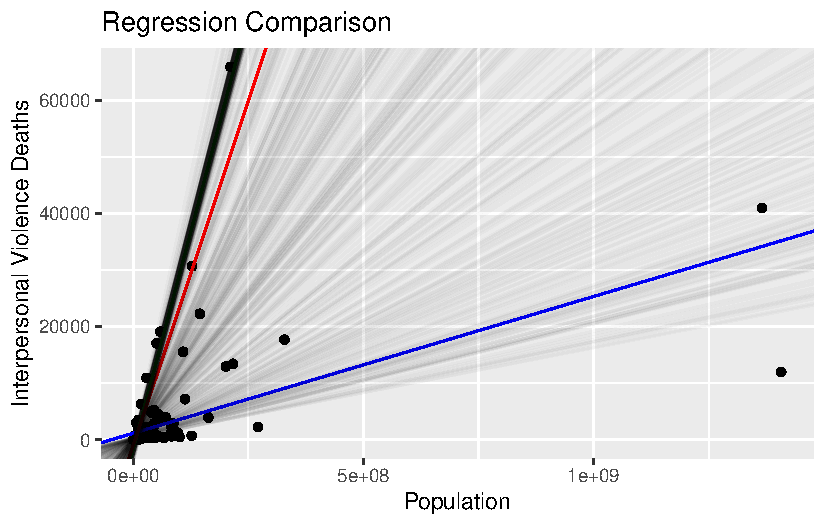
\includegraphics{Bootstrapping-Group-Report_files/figure-pdf/unnamed-chunk-24-1.pdf}

}

\end{figure}

A comparison of the regression lines further solidify the results shown
in the table. The sample model (green) and Bootstrap model (red) usually
fall closely together on the line. Since the Bootstrap models are
created using the same set of data as the initial sample this is
expected. With this specific data set, how close the population model
(blue) falls to the other two is highly variable. Since the results are
different every time the models are created it's possible that the
Bootstrap model could fit the true population almost identically. More
interesting, to visualize the variability, all Bootstrap models created
are graphed (black). This shows the extreme values that can occur with
this dataset.

\begin{Shaded}
\begin{Highlighting}[]
\CommentTok{\# Create a histogram of the intercepts found from the Bootstrap method}
\NormalTok{interceptHistogram }\OtherTok{\textless{}{-}} \FunctionTok{ggplot}\NormalTok{() }\SpecialCharTok{+} 
                      \FunctionTok{aes}\NormalTok{(boot\_estimated\_intercepts) }\SpecialCharTok{+}
                      \FunctionTok{geom\_histogram}\NormalTok{() }\SpecialCharTok{+}
                      \FunctionTok{ylab}\NormalTok{(}\StringTok{"Count"}\NormalTok{) }\SpecialCharTok{+}
                      \FunctionTok{xlab}\NormalTok{(}\StringTok{"Bootstrap Intercepts"}\NormalTok{)}

\CommentTok{\# Create a histogram of the regression parameter found from the Bootstrap }
\CommentTok{\# method}
\NormalTok{parameterHistogram }\OtherTok{\textless{}{-}} \FunctionTok{ggplot}\NormalTok{() }\SpecialCharTok{+} 
                      \FunctionTok{aes}\NormalTok{(boot\_estimated\_regressionparameters) }\SpecialCharTok{+}
                      \FunctionTok{geom\_histogram}\NormalTok{() }\SpecialCharTok{+}
                      \FunctionTok{ylab}\NormalTok{(}\StringTok{"Count"}\NormalTok{) }\SpecialCharTok{+}
                      \FunctionTok{xlab}\NormalTok{(}\StringTok{"Bootstrap Regression Parameters"}\NormalTok{)}

\CommentTok{\# Display plots side by side}
\FunctionTok{grid.arrange}\NormalTok{(interceptHistogram, parameterHistogram, }\AttributeTok{ncol =} \DecValTok{2}\NormalTok{)}
\end{Highlighting}
\end{Shaded}

\begin{figure}[H]

{\centering 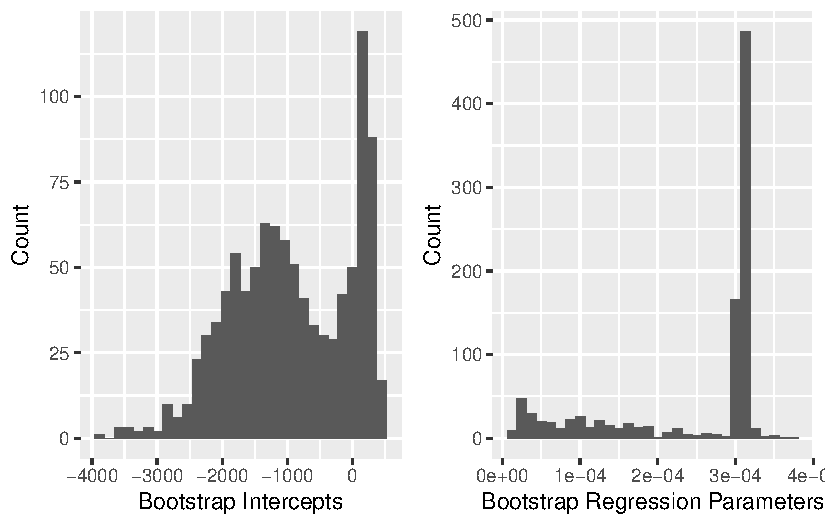
\includegraphics{Bootstrapping-Group-Report_files/figure-pdf/unnamed-chunk-26-1.pdf}

}

\end{figure}

Again, similar to the means and standard deviations found in the first
experiment, the intercepts appear to follow a normal distribution. The
regression parameters usually do not appear to follow a normal
distribution.

\hypertarget{conclusion}{%
\subsubsection{Conclusion}\label{conclusion}}

In the first experiment, the population mean and standard deviation were
estimated using the Bootstrap method. After 1,000 new samples were
created and the means and standard deviations from every sample saved,
they were used to create a 95\% confidence interval for the population
mean and standard deviations. Using those confidence intervals, the true
population values could be compared. It was found that the confidence
interval for both the mean and standard deviation fell within the
confidence intervals. Lastly, we could visualize that the estimated
means followed a normal distribution.

In the second experiment the simple linear regression model to estimate
the number of deaths caused by interpersonal violence on the country
population was analyzed for variability in the model. Again, using 1,000
new samples, a model was fit for every sample created and the intercepts
and regression parameters were saved. The average of all 1,000
intercepts and regression parameters were found to create the Bootstrap
model. This model was then compared against the model created using the
full population data and the model created using the initial sample
data. It was found that the Bootstrap model usually follows the sample
model more closely than the full population model. A graph was presented
to show the difference between the three models, along with displaying
all models created as part of the Bootstrap method.

These two experiments scratch the surface of demonstrate the usefulness
of the Bootstrap method. The population mean, standard deviation, and
distribution of the rate of death caused by cardiovascular diseases were
able to be successfully estimated. The model of deaths caused by
interpersonal violence on population was able to be analyzed to show it
has high variability.

\hypertarget{references}{%
\subsection*{References}\label{references}}
\addcontentsline{toc}{subsection}{References}

\hypertarget{refs}{}
\begin{CSLReferences}{1}{0}
\leavevmode\vadjust pre{\hypertarget{ref-worldbank}{}}%
2022. \url{https://data.worldbank.org/indicator/SP.POP.TOTL}.

\leavevmode\vadjust pre{\hypertarget{ref-lasso}{}}%
Chatterjee, A., and S. N. Lahiri. 2011. {``Bootstrapping Lasso
Estimators.''} \emph{Journal of the American Statistical Association}
106 (494): 608--25. \url{http://www.jstor.org/stable/41416396}.

\leavevmode\vadjust pre{\hypertarget{ref-chavez_2022}{}}%
Chavez, Ivan. 2022.
\url{https://www.kaggle.com/datasets/ivanchvez/causes-of-death-our-world-in-data}.

\leavevmode\vadjust pre{\hypertarget{ref-smooth}{}}%
Dwornicka, Renata, Andrii Goroshko, and Jacek Pietraszek. 2019. {``The
Smoothed Bootstrap Fine-Tuning.''} \emph{System Safety: Human -
Technical Facility - Environment} 1 (1): 716--23.
\url{https://doi.org/doi:10.2478/czoto-2019-0091}.

\leavevmode\vadjust pre{\hypertarget{ref-efron1}{}}%
Efron, B. 1979. {``Bootstrap Methods: Another Look at the Jackknife.''}
\emph{The Annals of Statistics} 7 (1): 1--26.
\url{http://www.jstor.org/stable/2958830}.

\leavevmode\vadjust pre{\hypertarget{ref-efron2}{}}%
Efron, Bradley. 1981. {``Nonparametric Estimates of Standard Error: The
Jackknife, the Bootstrap and Other Methods.''} \emph{Biometrika} 68 (3):
589--99. \url{http://www.jstor.org/stable/2335441}.

\leavevmode\vadjust pre{\hypertarget{ref-introduction}{}}%
Hossain, Mohammad. 2000. {``Bootstrapping -- an Introduction and Its
Applications in Statistics.''} \emph{Bangladesh Journal of Scientific
Research} 18 (January): 75--88.

\leavevmode\vadjust pre{\hypertarget{ref-difficult}{}}%
MD, MS, PhD MD, Jason Haukoos, and Roger Lewis. 2005. {``Advanced
Statistics: Bootstrapping Confidence Intervals for Statistics with
{`Difficult'} Distributions.''} \emph{Academic Emergency Medicine} 12
(April): 360--65. \url{https://doi.org/10.1197/j.aem.2004.11.018}.

\leavevmode\vadjust pre{\hypertarget{ref-confidenceintervals}{}}%
Puth, Marie-Therese, Markus Neuhäuser, and Graeme D. Ruxton. 2015. {``On
the Variety of Methods for Calculating Confidence Intervals by
Bootstrapping.''} \emph{Journal of Animal Ecology} 84 (4): 892--97.
https://doi.org/\url{https://doi.org/10.1111/1365-2656.12382}.

\leavevmode\vadjust pre{\hypertarget{ref-bayesian}{}}%
Rubin, Donald B. 1981. {``The Bayesian Bootstrap.''} \emph{The Annals of
Statistics} 9 (1): 130--34. \url{http://www.jstor.org/stable/2240875}.

\leavevmode\vadjust pre{\hypertarget{ref-withr}{}}%
Sillabutra, Jutatip, Prasong Kitidamrongsuk, Chukiat Viwatwongkasem,
Chareena Ujeh, Siam Sae-tang, and Khanokporn Donjdee. 2016.
{``Bootstrapping with r to Make Generalized Inference for Regression
Model.''} \emph{Procedia Computer Science} 86: 228--31.
https://doi.org/\url{https://doi.org/10.1016/j.procs.2016.05.103}.

\leavevmode\vadjust pre{\hypertarget{ref-assumptions}{}}%
Totty, Njesa, James Molyneux, and Claudio Fuentes. 2021. {``The
Importance of Discussing Assumptions When Teaching Bootstrapping.''}
arXiv. \url{https://doi.org/10.48550/ARXIV.2112.07737}.

\end{CSLReferences}



\end{document}
